\documentclass[12pt,a4paper]{article}

% Quelques options d'encodage, de langues et de format du document
\usepackage[utf8]{inputenc}
\usepackage[T1]{fontenc}
\usepackage[english]{babel}
\usepackage[top=2cm, bottom=3cm, left=1.75cm, right=1.75cm]{geometry}
\usepackage{setspace}
\usepackage{amsmath}
\usepackage{graphicx} % Pour la commande "\includegraphics"
\usepackage{hyperref} % Pour la commande "\url"

\pagenumbering{gobble}

\usepackage{tikz}
\usetikzlibrary{arrows.meta, positioning}

\begin{document}

\begin{center}
  \begin{tabular}{|p{0.2\textwidth}|p{0.75\textwidth}|}
    \hline
    {
    \vspace{0cm} % without it, bugs, don't know why?
    \centerline{\includegraphics[width=\linewidth]{tp-ipp.png}}
    }
    & {
      \vspace{0cm} % same here
      \centering
      \large
      {\hfill January, 2025}
      
      \vspace*{.5cm}
      \textbf{APM\_5AI29\_TP}
      
      \vspace*{.5cm}
      \setstretch{1.5}
      {\Large\textbf{Language Models and Structured Data}}
      
      \vspace*{.5cm}
      Mid-term Project Report

      \vspace*{1cm}
      %{\hfill\href{http://teaching.simplicitytheory.science}{teaching.simplicitytheory.science}}
      } \\
    \hline
  \end{tabular}
\end{center}

\noindent Acronym of the Team: FITJ\\
Name:	Fidelin-Durand Julian, Isabelle Neuveu, Tao Guinot, Florian Morel

{\centering\rule{\linewidth}{.5pt}}


%\maketitle
\begin{center}
\section*{Text To SQL}
\end{center}
\section*{Abstract}

We present here  3-step method to implement an agent capable of generating SQL queries from a user's question.

We first introduce the problem statement to then present the overall architecture. We present experimentation done so far and discussions. 

\section*{Problem Statement}

Chatting with data has been the most in demand application of LLMs past year, enterprises spending on GenAI increased sixfold in 2024, while it reached \$2.3 billion in 2023, enterprises are now looking for strong ROI and an important part of them are considering improving operation efficiency and data retrieval as the main criteria of investment \cite{MarketAnalysis} \cite{DeloitteResearch}.

Frameworks such as langchain of llama index have made simple to connect with SQL databases to write basic queries. But moving from basic to more advanced queries remain challenging, even more for smaller models adopted on premise by companies. Enterprises are looking for agents which they can chat with. Instead of groing from no automation to full automation (chatting with data directly), it is important to take a look at semi automation to understand what tasks the agent is actually performing, in our case translating a user's query to a SQL query.

Furthermore, breaking down the whole agent process may mitigate associated risks such as operational risks, data privacy risks, security risks or financial risks; being mostly due to the database access and the SQL query execution bypassing the user's correction.
\\

We present here a 3-step method to implement an agent capable at generating SQL queries from a user's question that would be usable in a production pipeline:
\begin{enumerate}
    \item Zero-shot and prompt engineered LLM evaluation (small general models and SQL-pretrained models)
    \item Fine tuned LLM, how good can they generalize ?
    \item Agent-based architecture and Retrieval-Augmented Generation
\end{enumerate}


\section*{Method/Overall Architecture}

As described earlier, our method will consist in 3 steps.
\subsection*{Zero-shot and prompt engineering}

In order to compare different ways to obtain the expected SQL queries, we decided to test three models, one general "Mistral" and two specifically trained to generate code "IBM-Granite" and "SQLcoder". We gave a prompt with the schema of the database as inputs. \\

The schema of our database is retrieved in the following format:  
Each table is represented as:  
\text{table\_name}: \text{column1 (type)}, \text{column2 (type)},
where each column is defined by its name and data type in parentheses, and tables are separated by \textbf{|}.  
For example, in the \textbf{concert\_singer} database, the schema is structured as follows:  
\textit{Stadium ID (number), Location (text), Name (text), Capacity (number), Highest (number), Lowest (number), Average (number) | singer : Singer ID (number), Name (text), Country (text), Song Name (text), Song release year (text), Age (number), Is male (others) | concert : concert ID (number), concert Name (text), Theme (text), Stadium ID (text), Year (text) | singer in concert : concert ID (number), Singer ID (text)}\\



We chose three approaches: the zero-shot prompt and the few-shot prompt, and the schema link prompt to witness if it makes any difference for the models. As an example of engineered prompts we have:\\
\\
\textbf{- Zero-shot prompt:} \\
\\
\textit{"Reply the SQL query only, without any comment, using this schema: {schema} to the question: How many singers do we have?
SQL QUERY:"}\\
\\
\textbf{- Few-shot prompt:} \\
\\
\textit{"You are an assistant specializing in generating SQL queries. The database is organized into several tables, each of which is described in the following form:
- **Table name** followed by a colon (`:`)
- **List of columns** with each column :
 - Its name
 - Its data type (`number` for a number, `text` for a character string, etc.)
 This is the database schema:{schema}".} \\
-----------\\
\textit{EXAMPLES\\
Question: What is the 3 most common cloud cover rates in the region of zip code 94107?\\
SELECT cloud cover FROM weather WHERE zip code = 94107 GROUP BY cloud cover ORDER BY COUNT (*) DESC LIMIT 3\\
Question: Count the number of schools.\\
SELECT count(*) FROM school\\
Question: What are the names of all campuses located at Chico?\\
SELECT campus FROM campuses WHERE LOCATION = "Chico"\\
Question: Which colleges does each player with a name that starts with the letter D who tried out go to?\\
SELECT T1.cName FROM tryout AS T1 JOIN player AS T2 ON T1.pID = T2.pID WHERE T2.pName LIKE 'D\%'\\
Question: What are the names of all the players who received a yes during tryouts, and also what are the names of their colleges?\\
SELECT T1.pName, T2.cName FROM player AS T1 JOIN tryout AS T2 ON T1.pID = T2.pID WHERE T2.decision = 'yes'\\
-----------\\
QUESTION: What is the average, minimum, and maximum age for all French singers?\\
SQL QUERY:}\\

\textbf{- Schema Linking  prompt:} \\


We implement an \texttt{extract\_schema\_links} function that takes as input a question and a schema, then identifies table and column names in the SQL schema that match words from the user's question. It normalizes the text by converting it to lowercase and handling variations. The function then checks if any table or column names appear in the question; if a match is found, it stores the table name in \texttt{schema\_links} as a key and maps the column name to its corresponding table.  

For example, given the question:  
\begin{quote}
    \textit{"Find all employees and their salaries"}
\end{quote}
and the schema:  
\begin{quote}
    \textit{"employees: id, name, salary | departments: id, name"}
\end{quote}
the output will be the dictionary:  
\begin{quote}
    \texttt{\{'employees': 'employees', 'salary': 'employees'\}}
\end{quote}

Then, the \texttt{generate\_sql\_with\_schema\_links} function creates a prompt for SQL query generation using these schema links:
\begin{verbatim}
schema_links = extract_schema_links(question, schema)

prompt_schema_linking = (
    "You are an SQL assistant. The database contains the following tables:\n\n"
    "{schema}\n\n"
    "The following question must be converted into SQL. Make sure to correctly associate the terms "
    "from the question with the corresponding columns and tables.\n\n"
    "Question: {question}\n\n"
    "The identified matches between the question and the schema are:\n"
    "{schema_links}\n\n"
    "Generate the SQL query taking these correspondences into account:\nSQL:")
\end{verbatim}


\subsection*{Fine-Tuning LLM}
The second step method will consist of fine tuning an LLM on the provided \textit{\href{https://huggingface.co/datasets/richardr1126/spider-schema/viewer?row=1}{dataset}}, composed of questions, corresponding queries, and tables' schema.
\\
For now, this step has been left to explore.
\\
Fine-tuning is a training technique used to adapt a pre-trained Large Language Model (LLM) to a specific task. Instead of training a model from scratch—which is costly in terms of data and computation—fine-tuning adjusts the weights of an existing model by re-training it on a task-specific dataset. There are various fine-tuning approaches, ranging from full model re-weighting to more lightweight methods. Each method has its own advantages and drawbacks, and we will present some of the techniques we applied in our project.\\
\\
\textbf{-Fine-Tuning with LoRA (Low-Rank Adaptation)}\\
\\
LoRA is designed to optimize efficiency by reducing the computational and memory costs of adapting a model. Instead of modifying all model weights directly, LoRA introduces low-rank adaptation matrices in specific layers—typically in the linear transformation layers of the attention mechanism.

During our experiments, we attempted multiple times to implement LoRA but encountered failures due to insufficient VRAM resources. We used an NVIDIA A100 GPU with 40GB of VRAM on Google Colab, but the available resources were not sufficient to successfully fine-tune the model.
\\
\textbf{-Fine-Tuning using MistralAI Plateforme}
To do so, we had to build training data with the right format. The Mistral plateforme for training requires samples written as jsonl files with the structure:
\begin{figure}
    \centering
    \includegraphics[width=0.8\linewidth]{mistral_fine_tuning.png}
    \caption{Mistral AI recommended structure}
    \label{fig:enter-label}
\end{figure}
Then the training file was provided to the plateforme, the learning rate suggested was $10^{-5}$ since only the structure (table, attribute) was to be learned.

\subsection*{Agent-based architecture}

An agent is an object aiming to choose a sequence of actions to take. In chains, those actions are hardcoded while agents use language models to determine which action to take and in which order. An agent built to interact with databse would look like this:

\begin{itemize}
    \item Itent classification is performed to better understand the user's query
    \item Text-to-SQL is often framed as Retrieval-Augmented Generation application, where context (table schema, examples queries, etc.) are retrieved to enhance the performance of the LLM to answer the question. 
    \item A set of validators can be ran followed by a self-correction agent to fix errors.
\end{itemize}

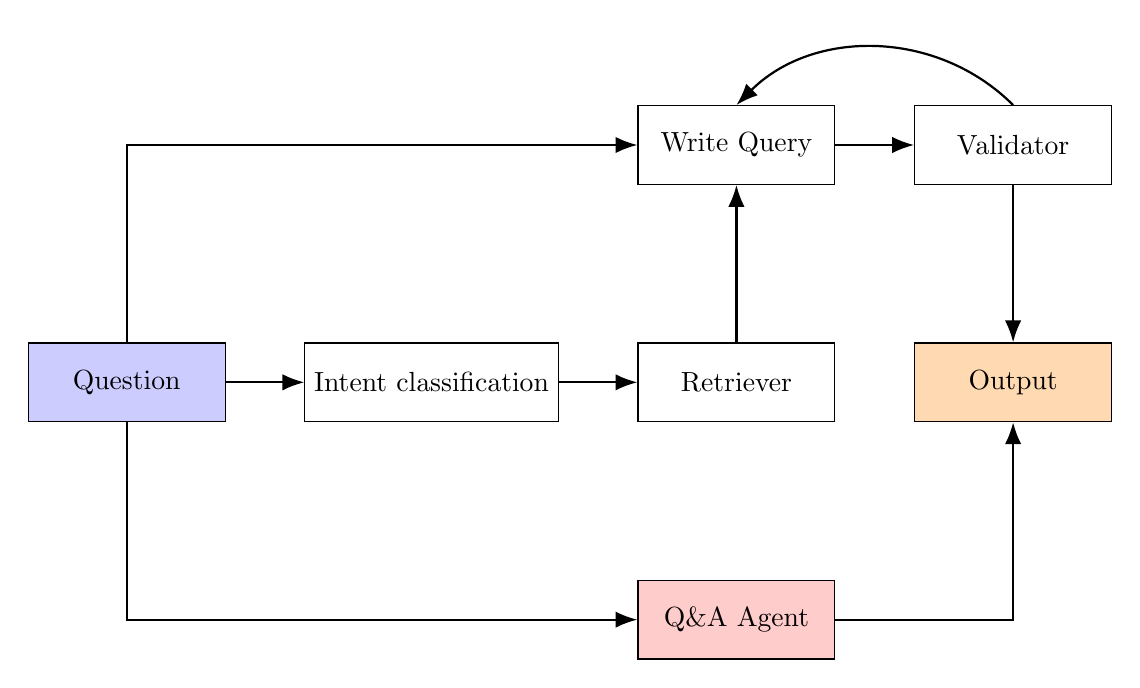
\begin{tikzpicture}[
    node distance=2cm and 1cm,
    every node/.style={draw, align=center, minimum width=2.5cm, minimum height=1cm},
    arrow/.style={-{Latex[scale=1.2]}, thick}
]

% Nodes
\node (question) [fill=blue!20] {Question};
\node (classification) [right=of question] {Intent classification};
\node (retriever) [right=of classification] {Retriever};
\node (writequery) [above=of retriever] {Write Query};
\node (validator) [right=of writequery] {Validator};
\node (output) [below=of validator, fill=orange!30] {Output};
\node (qanda) [below=of retriever, fill=red!20] {Q\&A Agent};

% Arrows
\draw [arrow] (question) -- (classification);
\draw [arrow] (classification) -- (retriever);
\draw [arrow] (retriever) -- (writequery);
\draw [arrow] (writequery) -- (validator);
\draw [arrow] (validator) -- (output);

% Edge arrows with 90° angles
\draw [arrow] (question.north) -- ++(0,0.5) |- (writequery.west);  % Arrow to Write Query
\draw [arrow] (question.south) -- ++(0,-0.5) |- (qanda.west);     % Arrow to Q&A Agent
\draw [arrow, bend right=45] (validator.north) to (writequery.north); % Bended arrow

% Arrow with 90° angle from Q&A Agent to Output
\draw [arrow] (qanda.east) -| (output.south); % 90° angle arrow (right then up)

\end{tikzpicture}

It is important to mention that because some table can be incomplete or doesn't necessarily contain explicit column names, a certification effort has to be pursued to describe the databases. Those description can consist in human description of table and their fields, an AI description, jargon, query examples or description status.

Since this is not the aim of our work, we will focus on building a simpler yet effective agent.
\vspace{1cm}

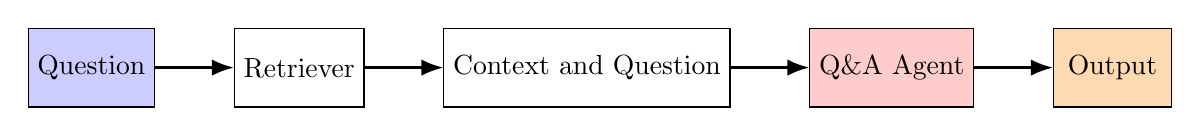
\begin{tikzpicture}[
    node distance=1cm and 1cm,
    every node/.style={draw, align=center, minimum width=1.5cm, minimum height=1cm},
    arrow/.style={-{Latex[scale=1.2]}, thick}
]

% Nodes
\node (question) [fill=blue!20] {Question};
\node (retriever) [right=of question] {Retriever};
\node (contextquestion) [right=of retriever] {Context and Question};
\node (qanda) [right=of contextquestion, fill=red!20] {Q\&A Agent};
\node (output) [right=of qanda, fill=orange!30] {Output};


% Arrows
\draw [arrow] (question) -- (retriever);
\draw [arrow] (retriever) -- (contextquestion);
\draw [arrow] (contextquestion) -- (qanda);
\draw [arrow] (qanda) -- (output);

\end{tikzpicture}

\subsection*{Evaluation}
The goal is to produce a SQL query as close as a groundtruth query provided in a train dataset. It is important to notice that two different queries can lead to the same result with different performance when ran toward a SQL database.

To evaluate the LLM performance, we set different metrics:
\begin{enumerate}
    \item Keyword metric
    \item Identifier metric
    \item Logical metric
\end{enumerate}

\\
Let us review those metrics.

\subsubsection*{Keyword metric}

The \texttt{keyword\_score} is a metric that evaluates the similarity between the keywords of two SQL queries (SELECT, WHERE, FROM, GROUP BY...). Doing an analogy with a binary classification problem we can compute the F1-score as follows :

\[
\text{F1 score} = \frac{TP}{TP + 0.5 \times (FP + FN)}
\]

\noindent Where:

\begin{itemize}
  \item \( TP \) (True Positives) is the number of keywords that appear in both the predicted query and the ground truth query.
  \item \( FP \) (False Positives) is the number of keywords present in the predicted query but not in the ground truth query.
  \item \( FN \) (False Negatives) is the number of keywords present in the ground truth query but not in the predicted query.
\end{itemize}

\noindent The \texttt{keyword\_score} ranges from 0 to 1:
\begin{itemize}
  \item A score of 1 indicates perfect overlap in the keywords between the predicted and ground truth queries.
  \item A score of 0 indicates no overlap in keywords.
\end{itemize}

\subsubsection*{Identifier metric}

The \texttt{identifier\_score} is a metric that compares the identifiers (such as table names, column names, max rows to return) between two queries. The principle is very similar to that of the keyword metric.

\begin{enumerate}
    \item Both queries are normalized and split at the SQL keyword level. \\ (example : SELECT name, age / FROM client / WHERE client.age > 18/ LIMIT 5)
    \item The F1 score is calculated for the identifiers inside each split (i.e. identifiers following each SQL keyword).
    \item The F1 scores are averaged to finally have a single value in $[0, 1]$ for the pair of queries.
\end{enumerate}

With the \texttt{identifier\_score}, we can check if the model is able to get the relevant attributes from the relevant tables, without considering the position of the words in a given SQL query.
For instance : '\texttt{SELECT name, age}' is equivalent to '\texttt{SELECT age, name}'.

\subsubsection*{Logical metric}




The Logical metric, or \texttt{equivalence\_score} method, is designed to return a numerical score representing how similar a generated SQL query is to a groundtruth query, based on the evaluation of an orchestrator LLM. This score is computed by invoking a separate model that compares the two queries and returns a score.
\\
\\
\textbf{Parameter}
\begin{itemize}
    \item \texttt{generated\_query}: A SQL query generated by the model based on a user's question.
    \item \texttt{query}: The groundtruth SQL query, which serves as the reference for comparison.
    \item \texttt{score\_prompt}: A prompt template used to ask the orchestrator LLM to provide a score.
\end{itemize}
\\
\textbf{Explanation}
\\
The method is aiming at returning a score between 0 and 1 and give some explanation of the result. The numerical score is found from the LLM answer with the regular expression pattern \texttt{\textbackslash s*([0-9]*\.?[0-9]+)}.
\\

\textbf{Return Values}
\\
The method returns a tuple containing:
\begin{itemize}
    \item A \texttt{float} representing the equivalence score between the two queries.
    \item A \texttt{str} explaining the score, which might include further details about the comparison.
\end{itemize}


score\_prompt = """Determine the degree of logical equivalence between the two SQL queries, assuming the same schema, data, and execution environment. Provide a score between 0 and 1, where:
\\
- 1: Fully logically equivalent (queries produce identical results under all circumstances).
\\
- 0: Completely different (queries are logically unrelated or produce entirely different results).
\\
- Scores between 0 and 1 should reflect partial equivalence, considering factors such as:
\\
- Differences in filters, conditions, or joins that partially overlap.
\\
- Minor variations in selected columns or formatting that do not affect the overall logic.
\\
- Similar intent but differing specifics in query structure.
\\
Explain your score briefly, highlighting key differences or similarities that influenced the rating.
Query 1:
\{query\}
Generated query:
\{generated\_query\}
Equivalence Score (0-1, with explanation):"""






\section*{Experimentation}
\subsection*{Results for Zero-shot and prompt engineering}

\begin{itemize}
  \item Dataset \& Dataset Statistics
  \end{itemize}
  The experiment was conducted on the dataset 'xlangai/spider', which was downloaded from Hugging Face. It consists of 8,034 question and SQL query pairs, divided into two splits: training (7,000) and validation (1,034). In addition to the questions and queries, the database name is provided, along with the token lists for both the queries and the questions. We evaluate the conversion of the question in natural language to an SQL query on all the validation dataset. We use zero-shot prompting and few-shot examples providing the database schema of each question in the prompt.
  
  \begin{itemize}
  \item Experimental Results based on Evaluation Metrics
  \end{itemize}
  We are testing with the three différents prompts the two pretrained models for generating SQL queries: \textbf{IBM Granite} and \textbf{ISQLCoder-7B-2}.
The key feature of the Granite model is its large scale, having been trained on 3 trillion tokens from 116 programming languages to develop a deep understanding of syntax. Additionally, a second training phase with 500 billion high-quality tokens enhanced its reasoning and ability to follow instructions.
In contrast, SQLCoder-7B-2, based on CodeLlama-7B, is specifically designed for text-to-SQL tasks. It enables non-technical users to generate SQL queries for data analysis. Updated on Feb 7, 2024, it offers improved performance, especially for joins, but should only be used with read-only database access. In the table below, the value of the \textbf{compute metric} is displayed, which is the reference metric of our Spider dataset.\\

\begin{table}[h]
    \centering
    \small
    \begin{tabular}{|l|c|c|c|}
        \hline
        \textbf{Model} & \textbf{Zero shot} & \textbf{Few shot} & \textbf{Schema link} \\ \hline
        Granite model & 0.70 & 0.72 & 0.75 \\ \hline
        SQLCoder    & 0.65 & 0.65 & 0.63 \\ \hline
    \end{tabular}
    \caption{Value of compute metric for Granite model and SQLCoder.}
    \label{tab:evaluation_metrics}
\end{table}\\


Here, we observe the limitations of task-specific training and how larger models can outperform smaller, task-oriented models even in their specialized domain.
With few-shot prompting, the Granite model benefits from additional context, which helps it generate more accurate queries and reduces hallucinations. The schema linking further enhances the quality of the generated queries by ensuring the correct column names and structure are used, allowing the model to determine when a join is necessary.
However, SQLCoder does not benefit as much from prompt engineering due to its smaller size and its specialized training on specific types of prompts, which limits its adaptability.

\begin{itemize}
\item Experimental Results for Ministral model
\end{itemize}

To compare with the two models presented before, we also tested the ministral model, which is a general LLM, on the same task. The following results are obtained without specific training.

\begin{table}[h]
    \centering
    \begin{tabular}{|c|c|c|c|c|}
        \hline
         \textbf{Prompt}& \textbf{Valid} & \textbf{keyword}&\textbf{Identifier}& \textbf{results}\\
         \hline
         Zero shot& 1.0&0.965&0.445&0.223 \\
         Few shot& 1.0&0.97&0.551&0.605\\
         \hline
    \end{tabular}
    \caption{Results of Ministral without fine-tuning}
    \label{tab:my_label}
\end{table}
As it can be seen in the last column, the performance of the model are way lower than the specialized ones. Ministral seems to face difficulties when it comes to the understanding and re-use the schema of the database. It often makes mistakes in the naming of attributes (for example, "Country" is replaced by "Citizenship") but the few shot strategy enable it to perform way better. This leads to consider a fine-tuned model which learned the table and their attributes as well as the expected format of the gold answers. 
\section*{Conclusion}

Our evaluations involved generating SQL queries from text using the Granite model, which is specialized in code, by applying prompt engineering with the table description from our database. However, the results remain insufficient, particularly in terms of the identifier score.\\

Our future work will focus on refining our evaluation metrics and testing other models specialized in SQL that are less voluminous than the Granite model, which is trained on 116 programming languages. We will also explore less specialized models to compare their performance.
Furthermore, we observed that our dataset consists of pairs of natural language questions that are similar but phrased differently while expecting the same SQL query. This insight suggests that evaluating the robustness of our model could be valuable.\\

Finally, integrating all our databases into a Retrieval-Augmented Generation (RAG) system could enable the generation of more complex and accurate queries, involving multiple databases through joins. Additionally, we will explore agent-based architectures to further enhance query generation.

\section*{Bibliography}
\bibliographystyle{plain}
\bibliography{sample}


\end{document}
